% The 20 affine maps x -> ax+b of F_5, arranged by their parameters.
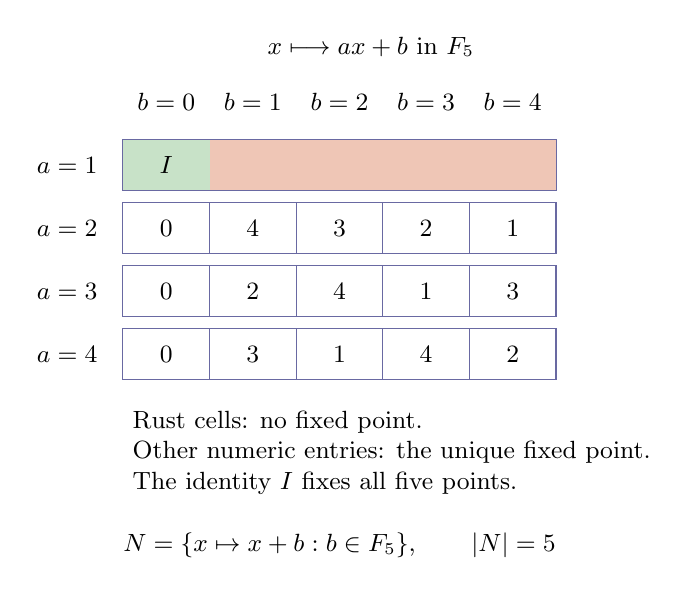
\begin{tikzpicture}[font=\small]
\node at (3.8,0.7) {$x\longmapsto ax+b$ in $\mathbb F_5$};
\foreach \b in {0,1,2,3,4}{\node at (1.2+1.1*\b,0) {$b=\b$};}
\foreach \a in {1,2,3,4}{
 \node[left] at (0.45,-0.8*\a) {$a=\a$};
 \foreach \b in {0,1,2,3,4}{
  \draw[MidnightBlue!65] (0.65+1.1*\b,-0.8*\a+0.32) rectangle (1.75+1.1*\b,-0.8*\a-0.32);
 }
}
\fill[ForestGreen!25] (0.65,-0.48) rectangle (1.75,-1.12);
\node at (1.2,-0.8) {$I$};
\foreach \b in {1,2,3,4}{
 \fill[BrickRed!20] (0.65+1.1*\b,-0.48) rectangle (1.75+1.1*\b,-1.12);
 \node at (1.2+1.1*\b,-0.8) {$\varnothing$};
}
% Unique fixed point is b/(1-a) modulo 5.
\foreach \a/\inv in {2/4,3/2,4/3}{
 \foreach \b in {0,1,2,3,4}{
  \pgfmathtruncatemacro{\fixed}{mod(\inv*\b,5)}
  \node at (1.2+1.1*\b,-0.8*\a) {$\fixed$};
 }
}
\node[align=left,anchor=north west] at (0.65,-3.8) {Rust cells: no fixed point.\\Other numeric entries: the unique fixed point.\\The identity $I$ fixes all five points.};
\node[below] at (3.4,-5.35) {$N=\{x\mapsto x+b:b\in\mathbb F_5\},\qquad |N|=5$};
\end{tikzpicture}
